\documentclass{article}
\usepackage[utf8]{inputenc}
\usepackage{tikz}
\usetikzlibrary{positioning}
\usetikzlibrary{shapes}

\begin{document}

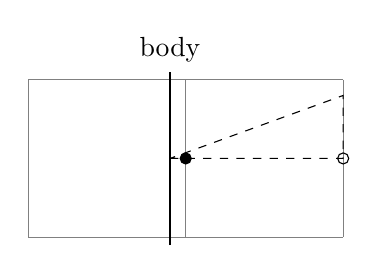
\begin{tikzpicture}
%grid
%horizontal
\draw[gray, thin] (-2,1) -- (2,1);
\draw[gray, thin] (-2,-1) -- (2,-1);
%vertical
\draw[gray, thin] (-2,1) -- (-2,-1);
\draw[gray, thin] (0,1) -- (0,-1);
\draw[gray, thin] (2,1) -- (2,-1);
%body
\draw[black, thick] (-0.2,-1.1) -- (-0.2,1.1) node[anchor=south] {body}; 
%triangle
\draw[black, dashed] (-0.2,0) -- (2,0) -- (2,0.8) -- cycle;
%nodes
\draw [black] (2.0,0) circle (2pt); %fluid
\filldraw [black] (0,0) circle (2pt);%hybrid

\end{tikzpicture}
\end{document}
